%!TEX root = /Users/louis/Documents/PhD/Deliverables/Thesis/thesis.tex

\chapter{Implementation}
\label{Implementation}
Section~\ref{sec:requirements_identification} identified requirements for structures and processes for managing co-evolution. In this chapter, the way in which this thesis approaches those requirements is described. Several related solutions were implemented, using domain-specific languages, automation and extensions to existing modelling technologies. Figure~\ref{fig:implementation_overview} summarises the structure of the chapter. To better support co-evolution and to overcome restrictions with existing modelling frameworks, a metamodel-independent syntax was devised and implemented, enabling model and metamodel decoupling and consistency checking (Section~\ref{sec:mmi_syntax}). To address some of the challenges faced in user-driven co-evolution, an OMG specification for an alternative, textual modelling notation was implemented (Section~\ref{sec:notation}). Model migration languages were identified, analysed and compared, leading to the derivation and implementation of a new model transformation language tailored for model migration and centred around a novel approach to relating source and target model elements (Section~\ref{sec:flock}). 

\begin{figure}[htbp]
  \begin{center}
    \leavevmode
    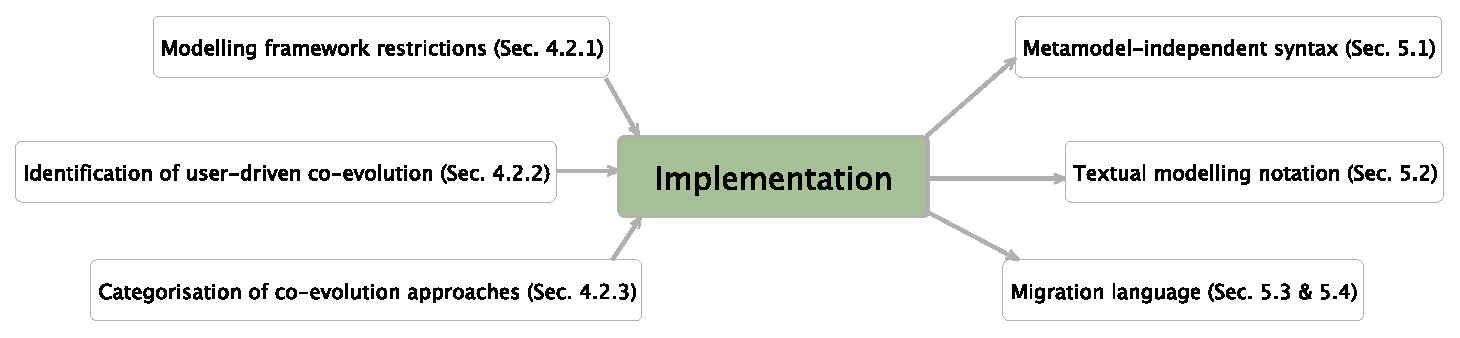
\includegraphics[width=12cm]{5.Implementation/overview.pdf}
  \end{center}
  \caption{Implementation chapter overview.}
  \label{fig:implementation_overview}
\end{figure}


\section{Metamodel-Independent Syntax}
\label{sec:mmi_syntax}
Section~\ref{subsec:modelling_framework_characteristics} discussed the way in which modelling frameworks implicitly enforce conformance. Because of this, modelling frameworks cannot be used to load non-conformant models, and provide little support for checking the conformance of a model with other metamodels or other versions of a metamodel. In Section~\ref{sec:requirements_identification}, these concerns lead to the identification of the following requirement: \emph{This thesis must investigate the extension of existing modelling frameworks to support the loading of non-conformant models and conformance checking of models against other metamodels.}

This section describes the way in which existing modelling frameworks load and store models using a metamodel-specific syntax. An alternative storage representation is motivated by highlighting the problems that a metamodel-specific syntax poses for managing and automating co-evolution. The way in which automatic consistency checking can be performed using the alternative storage representation is demonstrated. The work presented in this section was published in \cite{rose09enhanced}.


\subsection{Model Storage Representation}
Throughout a model-driven development process, modelling frameworks are used to load and store models. XML Metadata Interchange (XMI) \cite{xmi}, the OMG standard for exchanging MOF-based models, is the canonical model representation used by many contemporary modelling frameworks. XMI specifies the way in which models should be represented in XML.

An XMI document defines one or more namespaces from which type information is drawn. For example, XMI itself provides a namespace for specifying the version of XMI being used. Metamodels are referenced via namespaces, allowing the specification of elements that instantiate metamodel types.

As discussed in Section~\ref{subsec:modelling_framework_characteristics}, modelling frameworks bind a model to its metamodel using the underlying programming language. The metamodel defines the way in which model elements will be bound, and frequently, binding is strongly-typed: each metamodel type is mapped to a corresponding type in the underlying programming language.

Listing~\ref{lst:xmi} shows XMI for an exemplar model conforming to a metamodel that defines \texttt{Person} as a metaclass with three features: a string-valued \texttt{name}, an optional reference to a \texttt{Person}, \texttt{mother}, and another optional reference to a \texttt{Person}, \texttt{father}.

\begin{lstlisting}[caption=Exemplar person model in XMI, label=lst:xmi, language=XML]
<?xml version="1.0" encoding="ASCII"?>
<xmi:XMI xmi:version="2.0" xmlns:xmi="http://www.omg.org/XMI" xmlns:families="http://www.cs.york.ac.uk/families">
	<families:Person xmi:id="_xNSb8KfZEd,0dNl1iq3EdQ" name="Franz" mother="_6ef33ff010b31df8a39080" father="_F520cDaa0jN,i10s8xZp2a" />
	<families:Person xmi:id="_6ef33ff010b31df8a39080" name="Julie" />
	<families:Person xmi:id="_F520cDaa0jN,i10s8xZp2a" name="Hermann" />
</xmi:XMI>
\end{lstlisting}

The model shown in Listing~\ref{lst:xmi} contains three \texttt{Person}s, Franz, Julie and Hermann. Julie is the mother and Hermann is the father of Franz. The mothers and fathers of Julie and Hermann are not specified. On line 2, the XMI document specifies that the families namespace will be used to refer to types defined by the metamodel with the identifier: \url{http://www.cs.york.ac.uk/families}. Each person defines an XMI ID (a universally unique identifier), and a name. The IDs are used for inter-element references, such as for the values of the mother and father features.

Binding a model element involves instantiating, in the underlying programming language, the metamodel type, and populating the attributes of the instantiated object with values that correspond to those specified in the model. Because an XMI document refers to metamodel types and features by name, binding fails when a model does not conform to its metamodel. 


\subsection{Binding to a generic metamodel}
\label{subsec:binding}
For situations when a model does not conform to its metamodel, this thesis proposes an alternative deserialisation mechanism, which binds a model to a \emph{generic} metamodel. A generic metamodel reflects the characteristics of the metamodelling language and consequently every model conforms to the generic metamodel. Figure~\ref{fig:slot_model} shows a minimal version of a generic metamodel for MOF. Model elements are bound to \texttt{Object}, data values to \texttt{Slot}.

\begin{figure}[htbp]
  \centering
  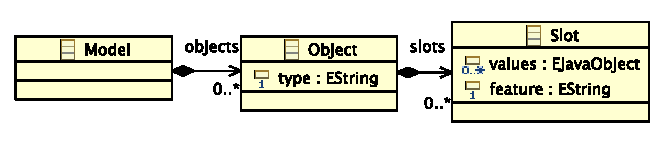
\includegraphics[width=3.3in]{5.Implementation/slot_model.pdf}
  \caption{A generic metamodel.}
  \label{fig:slot_model}
\end{figure}

Using the metamodel in Figure~\ref{fig:slot_model} in conjunction with MOF, conformance constraints can be expressed, as shown below. A minimal subset of MOF is shown in Figure~\ref{fig:minimal_mof}.

\begin{figure}[htbp]
  \centering
  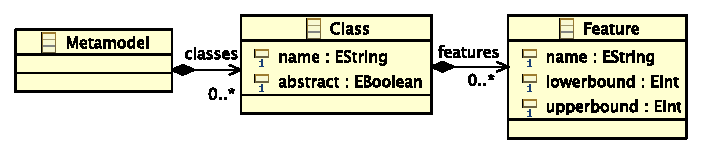
\includegraphics[width=3.3in]{5.Implementation/mof.pdf}
  \caption{Minimal MOF metamodel.}
  \label{fig:minimal_mof}
\end{figure}

The following constraints between metamodels (e.g. instances of MOF, Figure~\ref{fig:minimal_mof}) and models represented with a generic metamodel (e.g. instances of Figure~\ref{fig:slot_model}) can be used to express conformance:

\begin{enumerate}
	\item Each object's type must be the name of some non-abstract metamodel class.
	\item Each object must specify a slot for each mandatory feature of its type.
	\item Each slot's feature must be the name of a metamodel feature. That metamodel feature must belong to the slot's owning object's type.
	\item Each slot must be multiplicity-compatible with its feature. More specifically, each slot must contain at least as many values as its feature's lower bound, and at most as many values as its feature's upper bound.
  \item Each slot must be type-compatible with its feature.
\end{enumerate}

The way in which type-compatibility is checked depends on the way in which the modelling framework is implemented, and on its underlying programming language. EMF, for example, is implemented in Java and exposes some services for checking the type compatibility of model data with metamodel features. All metamodel features are typed and their types provide methods for determining the underlying programming language representation. Type compatibility checks can be implemented using these methods.

Conformance constraints vary over modelling languages. For example, Ecore, the modelling language of EMF, is similar to but not the same as MOF. For example, metamodel features defined in Ecore can be marked as transient (not stored to disk) and unchangeable (read-only). In EMF, extra conformance constraints are required which restrict the feature value of slots to only non-transient, changeable features.


\subsection{Example}
By binding a model not to the underlying programming languages types defined in its metamodel but to the generic metamodel presented in Figure~\ref{fig:slot_model}, conformance can be checked using the above constraints. Binding the exemplar XMI in Listing~\ref{lst:xmi} to the generic metamodel shown in Figure~\ref{fig:slot_model} produces three Objects, all with type ``Person''. Each class object contains a slot whose feature is name, one with the value ``Franz'', one with the value ``Julie'' and the other with the value ``Hermann''. The object containing the slot with value ``Franz'' contains two further slots: one whose feature is mother and whose value is a reference\footnote{The generic metamodel used in this thesis implements reference values using the proxy design pattern \cite{gamma95patterns}.} to the object that contains the name slot with the value ``Julie'' and one whose feature is father and whose value is a reference to the object containing ``Hermann''. A UML object diagram for this instantiation of the generic metamodel is shown in Figure~\ref{fig:generic_binding}. Instances of object (slot) are shaded grey (white).

\begin{figure}[htbp]
  \centering
  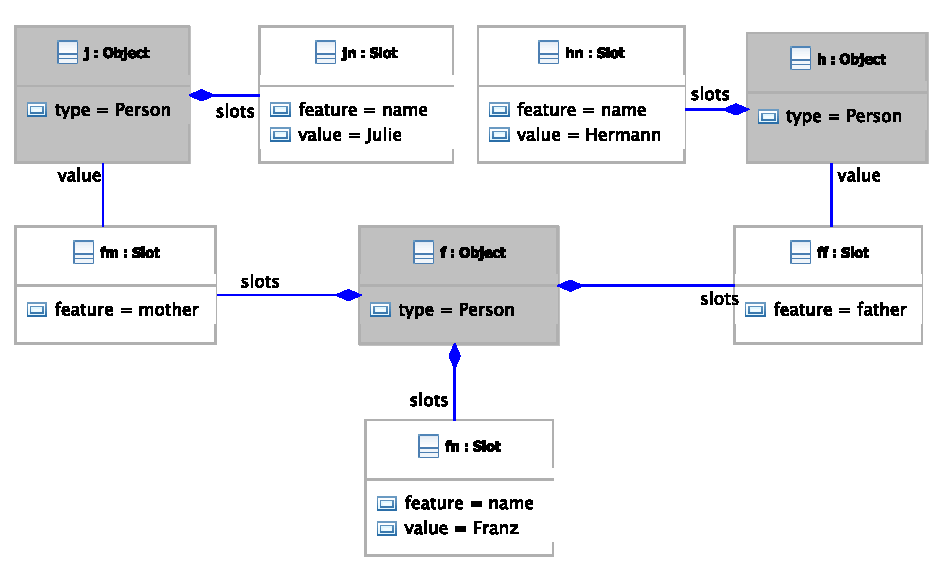
\includegraphics[width=4in]{5.Implementation/GenericBinding.pdf}
  \caption{Exemplar instantiation of generic metamodel.}
  \label{fig:generic_binding}
\end{figure}

After binding to the generic metamodel, the conformance of a model can be checked against any metamodel. Suppose the metamodel used to construct the XMI shown in Figure~\ref{fig:slot_model} has now evolved. The mother and father references have been removed, and replaced by a unifying parents reference. Conformance checking for the object representing Franz will fail because it defines slots for features ``mother'' and ``father'', which are no longer defined for the metamodel class ``Person''. More specifically, the model element representing Franz does not satisfy conformance constraint 4 from Section~\ref{subsec:binding}, which states that: each slot's feature must be the name of a metamodel feature. That metamodel feature must belong to the slot's owning object's type. 

\subsection{Applications}
As this section has shown, binding to a metamodel independent syntax is an alternative model deserialisation mechanism that can be used when a model no longer conforms to its metamodel and to check the conformance of a model with any metamodel. The metamodel independent syntax described in this section is used throughout this chapter to support other structures and processes for co-evolution.

In Section~\ref{sec:notation}, a textual modelling notation is integrated with the metamodel independent model representation discussed here. In Section~\ref{sec:flock}, a domain-specific language for migration uses metamodel independent syntax to perform partial migration by producing models that conform to a generic metamodel rather than their evolved metamodel.

\subsubsection{Automatic Consistency Checking}
\label{subsec:automatic_checking}
In addition to the applications outlined above, a metamodel independent syntax is particularly useful during metamodel installation. As discussed in Section~\ref{subsec:modelling_framework_characteristics}, metamodel developers do not have access to downstream models. Consequently, instances of a metamodel may become non-conformant after a new version of a metamodel plug-in is installed. By default, an EMF metamodel plug-in does not check conformance during plug-in installation and non-conformant models are only detected when the user attempts to load them.

To enable conformance checking as part of metamodel installation in EMF, the binding to a generic metamodel discussed above has been integrated with Concordance \cite{rose10concordance} in joint work with Dimitrios S. Kolovos, a lecturer in this department, Nicholas Drivalos, a research associate in this department and James R. Williams, a research student in this department.

Concordance provides a light-weight and efficient mechanism for resolving inter-model references, including the references between models and their metamodels. Concordance can be used to efficiently determine the instances of a metamodel, which is otherwise only possible with a brute force search of a development workspace.

The integration work involved extending Concordance such that, after the installation of a metamodel plug-in, models that conform to any previous version of the metamodel are identified. Those models are checked for conformance with the new metamodel. As such, conformance checking occurs automatically and during metamodel installation. Conformance problems are detected and reported immediately, rather than when the user next attempts to load an affected model. By integrating conformance checking with Concordance, improved scalability is achieved, as demonstrated in \cite{rose10concordance}. 


\section{Textual Modelling Notation}
\label{sec:notation}
% The Human-Usable Textual Notation is an OMG standard textual concrete syntax for the MOF metamodelling architecture. The notation is metamodel-independent -- it can be used with any model that conforms to any MOF-based metamodel. HUTN provides a human-usable means for visualising and specifying models, even when those models are inconsistent with their metamodel.
The analysis of co-evolution examples in Chapter~\ref{Analysis} highlighted two categories of process for managing co-evolution, developer-driven and user-driven. In the former, migration strategies are executable, while in the latter they are not. Performing user-driven co-evolution with modelling frameworks presents two key challenges that have not been explored by existing research. Firstly, user-driven co-evolution frequently involves editing the storage representation of the model, such as XMI. Model storage representations are typically not optimised for human use and hence user-driven co-evolution can be error-prone. Secondly, non-conformant model elements must be identified during user-driven co-evolution. When a multi-pass parser is used to load models, as is the case with EMF, not all conformance problems are reported at once, and user-driven co-evolution is an iterative process. In Section~\ref{sec:requirements_identification}, these challenges lead to the identification of the following requirement: \emph{This thesis must demonstrate a user-driven co-evolution process that enables the editing of non-conformant models without directly manipulating the underlying storage representation and provides a sound and complete conformance report for the original model and evolved metamodel.}

The remainder of this section describes a textual notation for models, which has been implemented for EMF, and discusses the way in which the notation has been integrated with the metamodel independent syntax described in Section~\ref{sec:mmi_syntax} to produce conformance reports. 


\subsection{Human-Usable Textual Notation}
\label{subsec:hutn}
The OMG's Human-Usable Textual Notation (HUTN) \cite{hutn} defines a textual modelling notation, which aims to conform to human-usability criteria \cite{hutn}. There is no current reference implementation of HUTN: the Distributed Systems Technology Centre's TokTok project (an implementation of the HUTN specification) is inactive (and the source code can no longer be found), whilst work on implementing the HUTN specification by Muller and Hassenforder \cite{muller05hutn} has been abandoned in favour of Sintaks \cite{sintaks}, which operates on domain-specific concrete syntax.

Model storage representations are often optimised to reduce storage space or to increase the speed of random access, rather than for human usability. By contrast, the HUTN specification states its primary design goal as human-usability and ``this is achieved through consideration of the successes and failures of common programming languages'' \cite[Section 2.2]{hutn}. The HUTN specification refers to two studies of programming language usability to justify design decisions. Because no reference implementation exists, the specification does not evaluate the human-usability of the notation. This thesis proposes that HUTN be used instead of XMI for user-driven co-evolution. Further discussion of the human-usability of HUTN is deferred to Chapter~\ref{Evaluation}.

Like the generic metamodel presented in Section~\ref{sec:mmi_syntax}, HUTN is a metamodel-independent syntax for 
MOF. In this section, the core syntax and key features of HUTN are introduced. The complete definition is available
in \cite{hutn}. To illustrate usage of the notation, the MOF-based metamodel of families in Figure \ref{fig:example-mm} is used. (A nuclear family ``consists only of a father, a mother, and children.'' \cite{nucleardef}).

\begin{figure}[htbp]
  \begin{center}
    \leavevmode
    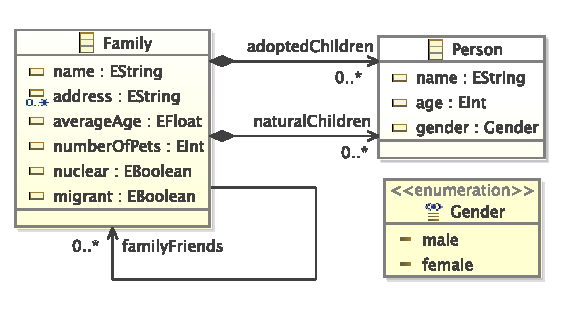
\includegraphics[scale=0.85]{5.Implementation/families.pdf}
  \end{center}
  \caption{Exemplar families metamodel. (Shading is irrelevant).}
  \label{fig:example-mm}
\end{figure}


\subsubsection{Basic Notation}
Listing \ref{lst:attributes} shows the construction of an \emph{object} in HUTN, here an instance of the Family class from Figure \ref{fig:example-mm}. Line 1 specifies the package containing the classes to be constructed (\texttt{FamilyPackage}) and a corresponding identifier (\texttt{families}), used for fully-qualifying references to objects (Section \ref{subsubsec:inter-package_references}). Line 2 names the class (\texttt{Family}) and gives an identifier for the object (\texttt{The Smiths}). Lines 3 to 7 define \emph{attribute values}; in each case, the data value is assigned to the attribute with the specified name. The encoding of the value depends on its type: strings are delimited by any form of quotation mark; multi-valued attributes use comma separators, etc.

The metamodel in Figure \ref{fig:example-mm} defines a \emph{simple reference} (familyFriends) and two \emph{containment references} (adoptedChildren; naturalChildren). The HUTN representation embeds a contained object directly in the parent object, as shown in Listing \ref{lst:containment}. A simple reference can be specified using the type and identifier of the referred object, as shown in Listing \ref{lst:non-contained}. Like attribute values, both styles of reference are preceded by the name of the meta-feature.

\begin{lstlisting}[caption=Specifying attributes with HUTN., label=lst:attributes, language=HutnFamilies]
FamilyPackage "families" {
    Family "The Smiths" {
        nuclear: true
        name: "The Smiths"
        averageAge: 25.7
        numberOfPets: 2
        address: "120 Main Street", "37 University Road"
    }
}
\end{lstlisting}

\begin{lstlisting}[caption=Instantiation of naturalChildren -- a HUTN containment reference., label=lst:containment, language=HutnFamilies]
FamilyPackage "families" {
    Family "The Smiths" {
        naturalChildren: Person "John" { name: "John" },
                                Person "Jo" { gender: female }
    }
}
\end{lstlisting}


\begin{lstlisting}[caption=Specifying a simple reference with HUTN., label=lst:non-contained, language=HutnFamilies]
FamilyPackage "families" {
    Family "The Smiths" {
        familyFriends: Family "The Does"
    }
    Family "The Does" {}
}
\end{lstlisting}


\subsubsection{Keywords and Adjectives}
While HUTN is unlikely to be as concise as a metamodel-specific concrete syntax, the notation does define syntactic shortcuts to make model specifications more compact. Shortcut use is optional, and the HUTN specification aims to make their syntax intuitive \cite[pg2-4]{hutn}. Two example notational shortcuts are described here, to illustrate some of the ways in which HUTN can be used to construct models in a concise manner.

When specifying a \emph{Boolean-valued attribute}, it is sufficient to simply use the attribute name (value \texttt{true}), or the attribute name prefixed with a tilde (value \texttt{false}). When used in the body of the object, this style of Boolean-valued attribute represents a \emph{keyword}. A keyword used to prefix an object declaration is called an \emph{adjective}. Listing \ref{lst:boolean} shows the use of both an attribute keyword (\texttt{\textasciitilde nuclear} on line 6) and adjective (\texttt{\textasciitilde migrant} on line 2).

\begin{lstlisting}[caption=Using keywords and adjectives in HUTN., label=lst:boolean, language=HutnFamilies]
FamilyPackage "families" {
    ~migrant Family "The Smiths" {}

    Family "The Does" {
        averageAge: 20.1
        ~nuclear
        name: "The Does"
    }
}
\end{lstlisting}


\subsubsection{Inter-Package References}
\label{subsubsec:inter-package_references}
To conclude the summary of the notation, two advanced features defined in the HUTN specification are discussed. The first enables objects to refer to other objects in a different package, while the second provides means for specifying the values of a reference for all objects in a single construct (which can be used, in some cases, to simplify the specification of complicated relationships).

\begin{lstlisting}[caption=Referencing objects in other packages with HUTN., label=lst:fullyqualified, language=HutnFamilies]
FamilyPackage "families" {
    Family "The Smiths" {}
}
VehiclePackage "vehicles" {
    Vehicle "The Smiths' Car" {
        owner: FamilyPackage.Family "families"."The Smiths"
    }
}
\end{lstlisting}

To reference objects between separate package instances in the same document, the package identifier is used to construct a fully-qualified name. Suppose a second package is introduced to the metamodel in Figure \ref{fig:example-mm}. Among other concepts, this package introduces a Vehicle class, which defines an owner reference of type Family. Listing \ref{lst:fullyqualified} illustrates the way in which the owner feature can be populated. Note that the fully-qualified form of the class utilises the names of elements of the metamodel, while the fully-qualified form of the object utilises only HUTN identifiers defined in the current document.

The HUTN specification defines name scope optimisation rules, which allow the definition above to be simplified to: \texttt{owner: Family "The Smiths"}, assuming that the VehiclePackage does not define a Family class, and that the identifier ``The Smiths'' is not used in the VehiclePackage block, or this HUTN document is configured to require unique identifiers over the entire document.


\subsubsection{Alternative Reference Syntax}
In addition to the syntax defined in Listings \ref{lst:containment} and \ref{lst:non-contained}, the value of references may be specified independently of the object definitions. For example, Listing \ref{lst:assocblock} demonstrates this alternate syntax by defining The Does as friends with both The Smiths and The Bloggs.

\begin{lstlisting}[caption=Using a reference block in HUTN., label=lst:assocblock, language=HutnFamilies]
FamilyPackage "families" {
    Family "The Smiths" {}
    Family "The Does" {}
    Family "The Bloggs" {}
    
    familyFriends {
        "The Does" "The Smiths"
        "The Does" "The Bloggs"
    }
}
\end{lstlisting}

Listing \ref{lst:associnfix} illustrates a further alternative syntax for references, which employs an infix notation. 

\begin{lstlisting}[caption=Using an infix reference in HUTN., label=lst:associnfix, language=HutnFamilies]
FamilyPackage "families" {
    Family "The Smiths" {}
    Family "The Does" {}
    Family "The Bloggs" {}
    
    Family "The Smiths" familyFriends Family "The Does";
    Family "The Smiths" familyFriends Family "The Bloggs";
}
\end{lstlisting}

The reference block (Listing~\ref{lst:assocblock}) and infix (Listing~\ref{lst:associnfix}) notations are syntactic variations on -- and have identical semantics to -- the reference notation shown in Listings \ref{lst:containment} and \ref{lst:non-contained}.


\subsubsection{Customisation via Configuration}
Some limited customisation of HUTN for particular metamodels can be achieved using \emph{configuration files}. Customisations permitted include a parametric form of object instantiation (not yet implemented); renaming of metamodel elements; giving default values for attributes; and stating an attribute whose values are used to infer a default identifier.


\subsection{Epsilon HUTN}
To investigate the extent to which HUTN can be used during user-driven co-evolution, an implementation was constructed. The implementation, Epsilon HUTN, makes extensive use of the Epsilon model management platform. Before presenting HUTN, it is necessary to revisit some details of the Epsilon \cite{kolovos09thesis} platform, which was introduced in Section~\ref{subsec:epsilon}.

\subsubsection{The Epsilon Platform}
Epsilon, a component of the Eclipse GMT project \cite{gmt}, provides infrastructure for implementing uniform and interoperable model management languages, for performing tasks such as model merging, model transformation and inter-model consistency checking. 

The core of the platform is the Epsilon Object Language (EOL) \cite{kolovos06eol}, a reworking and extension of OCL that includes the ability to update models, conditional and loop statements, statement sequencing, and access to standard I/O streams. EOL provides mechanisms for reusing sections of code, such as user-defined operators along with modules and import statements. The Epsilon task-specific languages are built atop EOL, giving highly efficient inheritance and reuse of features. Currently, these task-specific languages include support for model-to-model transformation (ETL \cite{kolovos08etl}), model-to-text transformation (EGL \cite{rose08egl}) and model validation (EVL \cite{kolovos08evl}).


\subsubsection{Implementation of Epsilon HUTN}
Epsilon HUTN uses the task-specific languages of Epsilon. Although any languages for model-to-model transformation 
(M2M), model-to-text transformation (M2T) and model validation could have been used, Epsilon's existing domain-specific languages are tightly integrated and inter-operable. Epsilon HUTN has been released as part of Epsilon, and includes development tools for Eclipse.

\begin{figure}[htbp]
  \begin{center}
    \leavevmode
    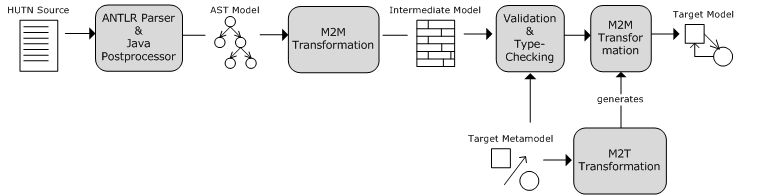
\includegraphics[scale=0.44]{5.Implementation/hutn_workflow.png}
  \end{center}
  \caption{The architecture of Epsilon HUTN.}
  \label{fig:architecture}
\end{figure}

Figure \ref{fig:architecture} outlines the workflow through Epsilon HUTN, from HUTN source text to instantiated target model. The HUTN model specification is parsed to an abstract syntax tree using a HUTN parser specified in ANTLR \cite{parr07antlr}. From this, a Java postprocessor is used to construct an instance of a simple AST metamodel (which comprises two meta-classes, Tree and Node). Using ETL, M2M transformations are then applied to produce an instance of the generic metamodel discussed in Section~\ref{sec:mmi_syntax}. Finally, a M2T transformation on the target metamodel, specified in EGL, produces a further M2M transformation, from the generic metamodel to the target model.

The workflow uses an extension of the generic metamodel defined in Section~\ref{sec:mmi_syntax}. Because the HUTN specification allows the use of packages, an extra element, \texttt{PackageObject}, was added to the generic metamodel. A \texttt{PackageObject} has a type, an optional identifier and contains any number of \texttt{Object}s. To avoid confusion with \texttt{PackageObjects}, the \texttt{Object} class in the generic metamodel was renamed to \texttt{ClassObject}.

Using two M2M transformation stages with the (extended) generic metamodel as an intermediary has two advantages. Firstly, the form of the AST metamodel is not suited to a one-step transformation. There is a mismatch between the features of the AST metamodel and the needs of the target model -- for example, between the Node class in the AST metamodel and classes in the target metamodel. If a one-step transformation were used, each transformation rule would need a lengthly guard statement, which is hard to understand and verify. Secondly, Section~\ref{sec:mmi_syntax} discussed a mechanism for binding XMI to the generic metamodel, which can be used in conjunction with the latter half of the Epsilon HUTN workflow (Figure~\ref{fig:architecture}) to generate HUTN from XMI. This process is discussed further in Section~\ref{subsec:migration_with_hutn}.

Throughout the remainder of this section, instances of the generic metamodel producing during the execution of the HUTN workflow are termed an \textit{intermediate model}. The two M2M transformations are now discussed in depth, along with a model validation phase which is performed prior to the second transformation.

\paragraph{AST Model to Intermediate Model}
Epsilon HUTN uses ETL for specifying M2M transformation. One of the transformation rules from Epsilon HUTN is shown in Listing \ref{lst:m2m}. The rule transforms a name node in the AST model (which could represent a package or a class object) to a package object in the intermediate model. The guard (line 5) specifies that a name node will only be transformed to a package object if the node has no parent (i.e. it is a top-level node, and hence a package rather than a class). The body of the rule states that the type, line number and column number of the package are determined from the text, line and column attributes of the node object. On line 11, a containment slot is instantiated to hold the children of this package object. The children of the node object are transformed to the intermediate model (using a built-in method, \verb|equivalent()|), and added to the containment slot.

\begin{lstlisting}[caption=Transformation rule (in ETL) to convert AST nodes to package objects., label=lst:m2m, language=ETL]
rule NameNode2PackageObject
    transform n : AntlrAst!NameNode
    to p : Intermediate!PackageObject {

    guard : n.parent.isUndefined()

    p.type := n.text;
    p.line := n.line;
    p.col  := n.column;

    var slot := new Intermediate!ContainmentSlot;
    for (child in n.children) {
        slot.objects.add(child.equivalent());
    }
    if (slot.objects.notEmpty()) {
        p.slots.add(slot);
    }
}
\end{lstlisting}

\paragraph{Intermediate Model Validation}
An advantage of the two-stage transformation is that contextual analysis can be specified in an abstract manner -- that is, without having to express the traversal of the AST. This gives clarity and minimises the amount of code required to define syntatic constraints.

\begin{lstlisting}[caption=A constraint (in EVL) to check that all identifiers are unique., label=lst:constraint, language=EVL]
context ClassObject {
    constraint IdentifiersMustBeUnique {
        guard: self.id.isDefined()
        check: ClassObject.allInstances()
                   .select(c|c.id = self.id).size() = 1;
        message: `Duplicate identifier: ' + self.id
    }
}
\end{lstlisting}

Epsilon HUTN uses EVL \cite{kolovos08evl} to specify verification, resulting in highly expressive syntactic constraints. An EVL constraint comprises a guard, the logic that specifies the constraint, and a message to be displayed if the constraint is not met. For example, Listing \ref{lst:constraint} specifies the constraint that every HUTN class object has a unique identifier.

In addition to the syntactic constraints defined in the HUTN specification, the conformance constraints described in Section~\ref{sec:mmi_syntax} are executed on the model at this stage. For this purpose, the conformance constraints are specified in EVL.

\paragraph{Intermediate Model to Target Model}
Because the contextual analysis is performed on the intermediate model, models conform to the target metamodel. In generating the target model from the intermediate model (Figure \ref{fig:architecture}), the transformation uses information from the target metamodel, such as the names of classes and features. A typical approach to this category of problem is to use a higher-order transformation on the target metamodel to generate the desired transformation. Epsilon HUTN uses a different approach: the transformation to the target model is produced by executing an EGL template on the target metamodel. EGL is a template-based text generation language. \verb|[% %]| tag pairs are used to denote dynamic sections, which may produce text when executed. Any code not enclosed in a \verb|[% %]| tag pair is included verbatim in the generated text.

Listing \ref{lst:generate} is the EGL template for a M2T transformation on the target metamodel; it generates the M2M transformation used for generating the target model. The loop beginning on line 1 iterates over each meta-class in the metamodel, producing a transformation rule to generate target model instances of that meta-class from class objects in the intermediate model. The template guard (line 6) specifies that only class objects of the same type as the meta-class be transformed by the current rule. For the body of the rule the template iterates over each structural feature of the current meta-class, and generates appropriate transformation code for populating the values of each structural feature from the slots on the class object in the intermediate model. The template body is omitted in Listing~\ref{lst:generate} because it contains a large amount of code for interacting with EMF, which is not relevant to this discussion.

\begin{lstlisting}[caption= Initial sections of the template (in EGL) for generating  rules (in ETL) to instantiate classes of the target metamodel., label=lst:generate, language=EOL]
[% for (class in EClass.allInstances()) { %]
rule Object2[%=class.name%]
  transform o : Intermediate!ClassObject
  to t : Model![%=class.name%] {

    guard: o.type = `[%=class.name%]'

    -- body omitted
  }
[% } %]
\end{lstlisting}

Presently, Epsilon HUTN can be used only to generate EMF models. Support for other modelling languages, such as MDR, would require different transformations between intermediate and target model. In other words, for each target modelling language, a new EGL template would be required. The transformation from AST to intermediate model is independent of the target modelling language and would not need to change.


\subsection{Migration with HUTN}
\label{subsec:migration_with_hutn}
Epsilon HUTN uses the generic metamodel (from Section~\ref{sec:mmi_syntax}) as an intermediary, facilitating transformation from XMI to HUTN (i.e. the inverse of the transformation discussed above): XMI is parsed to produce an instance of the generic metamodel, and an unparser (implemented using the visitor design pattern \cite{gamma95patterns}) generates HUTN source. In this manner, HUTN can be generated for any XMI document, regardless of whether the model described by the XMI conforms to its metamodel.\footnote{TODO: Somewhere, I need to discuss loss of information. (e.g. model element type information when a metaclass is removed)}

To demonstrate the way in which HUTN can be used to perform migration, the exemplar XMI shown in Listing~\ref{lst:xmi} is represented using HUTN in Listing~\ref{lst:non-conformant_hutn}. Recall that the XMI describes three Persons, Franz, Julie and Hermann. Julie and Hermann are the mother and father of Franz.

\begin{lstlisting}[caption=HUTN for people with mothers and fathers., label=lst:non-conformant_hutn, language=HutnFamilies]
Persons "kafkas" {
    Person "Franz"   { name: "Franz"   }
    Person "Julie"   { name: "Julie"   }
    Person "Hermann" { name: "Hermann" }
    
    Person "Franz" mother Person "Julie";
    Person "Franz" father Person "Hermann";
}
\end{lstlisting}

Note that, by using a configuration file to specify that a Person's name is taken from its identifier, the body of the Person objects could be omitted.

If the Persons metamodel now evolves such that mother and father are merged to form a parents reference, Epsilon HUTN reports conformance problems on the HUTN document, as illustrated by the screenshot in Figure~\ref{fig:hutn_conformance_reporting}.

\begin{figure}[htbp]
  \begin{center}
    \leavevmode
    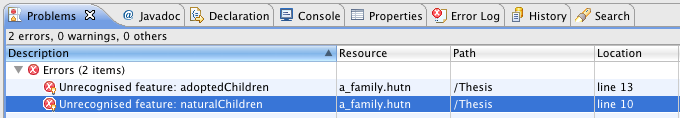
\includegraphics[scale=0.44]{5.Implementation/hutn_conformance_reporting.png}
  \end{center}
  \caption{Conformance problem reporting in Epsilon HUTN.}
  \label{fig:hutn_conformance_reporting}
\end{figure}

Resolving the conformance problems requires the user to change the feature named in the infix associations from mother (father) to parents. The Epsilon HUTN development tools provide content assistance, which might be useful in this situation. Listing~\ref{lst:conformant_hutn} shows a HUTN document that conforms to the metamodel defining parents rather than mother and father.

\begin{lstlisting}[caption=HUTN for people with parents., label=lst:conformant_hutn, language=HutnFamilies]
Persons "kafkas" {
    Person "Franz"   { name: "Franz"   }
    Person "Julie"   { name: "Julie"   }
    Person "Hermann" { name: "Hermann" }
    
    Person "Franz" parents Person "Julie";
    Person "Franz" parents Person "Hermann";
}
\end{lstlisting}


\subsection{Limitations}
Notwithstanding the power of genericity, there are situations where a metamodel-specific concrete syntax is preferable. An example of where HUTN is unhelpful arose when developing a metamodel for the recording of failure behaviour of components in complex systems, based on the work of \cite{wallace05modular}.

Failure behaviours comprise a number of expressions that specify how each component reacts to system faults, and there is an established concrete syntax for expressing failure behaviours. The failure syntax allows various shortcuts, such as the use of underscore to denote a wildcard. For example, the syntax for a possible failure behaviour of a component that receives input from two other components (on the left-hand side of the expression), and produces output for a single component is denoted:

\begin{eqnarray}\label{failure}
(\{\_\}, \{\_\}) \rightarrow (\{late\})
\end{eqnarray}

The above expression is written using a domain-specific syntax. In HUTN, the specification of these behaviours is less concise. For example, Listing \ref{lst:fptc-hutn} gives the HUTN syntax for failure behaviour (\ref{failure}), above.

\begin{lstlisting}[caption=Failure behaviour specified in HUTN., label=lst:fptc-hutn, language=FPTC]
Behaviour {
    lhs: Tuple {
        contents: IdentifierSet { contents: Wildcard {} },
                     IdentifierSet { contents: Wildcard {} }
    }

    rhs: Tuple {
        contents: IdentifierSet { contents: Fault "late" {} }
    }
}
\end{lstlisting}

The domain-specific syntax exploits two characteristics of failure expressions to achieve a compact notation. Firstly, structural domain concepts are mapped to symbols: tuples to parentheses and identifier sets to braces. Secondly, little syntactic sugar is needed for many domain concepts, as they define only one feature: a fault is referred to only by its name, the contents of identifier sets and tuples are separated using only commas.

In general, HUTN is less concise than a domain-specific syntax for metamodels containing a large number of classes with few attributes, and in cases where most attributes are used to define structural relationships among concepts. However, there might still be benefits from using HUTN in such cases, if the metamodel is likely to be modified frequently, of it the model does not yet have a formal metamodel.

\subsection{Summary}
In this section, HUTN was introduced and its syntax described. An implementation of HUTN for EMF, built atop Epsilon, was discussed. Integration of HUTN for the metamodel-independent syntax discussed in Section~\ref{sec:mmi_syntax} facilitates user-driven co-evolution with a textual modelling notation other than XMI, as demonstrated by the example above. The remainder of this chapter focuses on developer-driven co-evolution, in which model migration strategies are executable.


\section{Epsilon Flock}
\label{sec:flock}
Section~\ref{subsec:co-evolution_categorisation} discussed existing approaches to model migration, highlighting variation in the languages used for specifying migration strategies. In this section, migration strategy languages are compared, using the example of metamodel evolution given in Section~\ref{subsec:co-evo_example}. From this comparison, requirements for a domain-specific language for specifying and executing model migration strategies are derived (Section~\ref{subsec:analysis}) and an implementation is described (Section~\ref{subsec:flock_implementation}). This work described in this section was published in \cite{rose10flock}.


\subsection{Co-Evolution Example}
\label{subsec:co-evo_example}
Throughout this section, the following example of an evolution of a Petri net metamodel is used to discuss co-evolution and model migration. The same example has been used previously in co-evolution literature \cite{cicchetti08automating,garces09managing,wachsmuth07metamodel}.

\begin{figure}[bp]
	\centering
	\subfigure[Original metamodel.]
	{
	    \label{fig:original_mm}
	    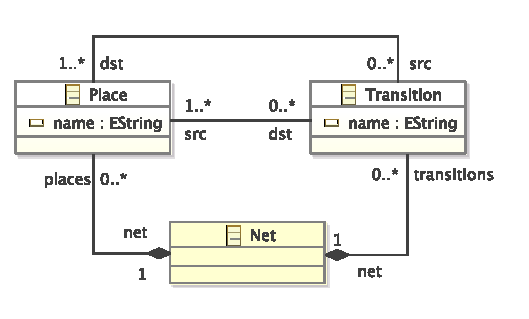
\includegraphics[width=4.75cm]{5.Implementation/petri_nets_step0.pdf}
	}
	\subfigure[Evolved metamodel.]
	{
	    \label{fig:evolved_mm}
	    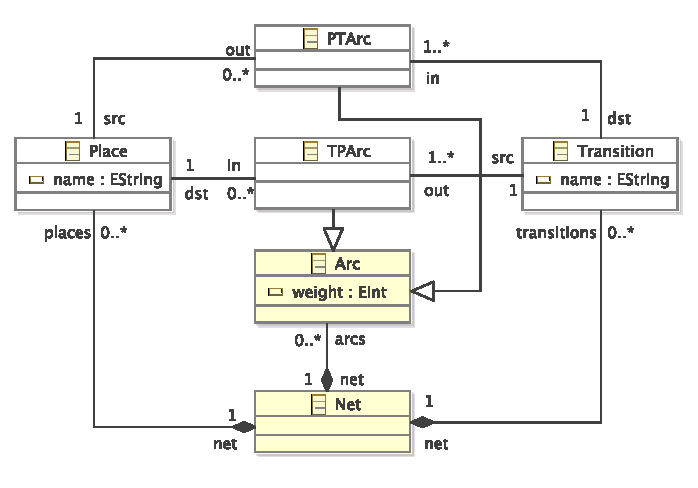
\includegraphics[width=6.25cm]{5.Implementation/petri_nets_step1.pdf}
	}
	\caption{Exemplar metamodel evolution. (Shading is irrelevant). Taken from \cite{rose10flock}.}
\label{fig:petri_nets_mms}
\end{figure}

In Figure~\ref{fig:original_mm}, a Petri \texttt{Net} comprises \texttt{Place}s and \texttt{Transition}s. A \texttt{Place} has any number of \texttt{src} or \texttt{dst} \texttt{Transition}s. Similarly, a \texttt{Transition} has at least one \texttt{src} and \texttt{dst} \texttt{Place}. In this example, the metamodel in Figure~\ref{fig:original_mm} is to be evolved so as to support weighted connections between \texttt{Place}s and \texttt{Transition}s and between \texttt{Transition}s and \texttt{Place}s.

The evolved metamodel is shown in Figure~\ref{fig:evolved_mm}. \texttt{Place}s are connected to \texttt{Transition}s via instances of \texttt{PTArc}. Likewise, \texttt{Transition}s are connected to \texttt{Place}s via \texttt{TPArc}. Both \texttt{PTArc} and \texttt{TPArc} inherit from \texttt{Arc}, and therefore can be used to specify a \texttt{weight}.

Models that conformed to the original metamodel might not conform to the evolved metamodel. The following strategy can be used to migrate models from the original to the evolved metamodel:

\begin{enumerate}
	\item For every instance, t, of \texttt{Transition}: 
	\subitem For every \texttt{Place}, s, referenced by the \texttt{src} feature of t: 
	\subsubitem Create a new instance, arc, of \texttt{PTArc}. 
	\subsubitem Set s as the \texttt{src} of arc. 
	\subsubitem Set t as the \texttt{dst} of arc. 
	\subsubitem Add arc to the \texttt{arcs} reference of the \texttt{Net} referenced by t.
	
	\subitem For every \texttt{Place}, d, referenced by the \texttt{dst} feature of t: 
	\subsubitem Create a new instance, arc, of \texttt{TPArc}. 
	\subsubitem Set t as the \texttt{src} of arc. 
	\subsubitem Set d as the \texttt{dst} of arc. 
	\subsubitem Add arc to the \texttt{arcs} reference of the \texttt{Net} referenced by t.
	
	\item And nothing else changes.
\end{enumerate}

Using the above example, the existing approaches for specifying and executing model migration strategies are now compared.


\subsection{Existing Approaches}
\label{subsec:existing_migration_languages}
Using the above example, the existing approaches for specifying and executing model migration strategies are now compared.

\subsubsection{Manual Specification with Model-to-Model Transformation}
\label{subsubsec:m2m}

A model-to-model transformation specified between original and evolved metamodel can be used for performing model migration. Part of the model migration for the Petri nets metamodel is codified with the Atlas Transformation Language (ATL) \cite{jouault05transforming} in Listing~\ref{lst:atl}. Rules for migrating \texttt{Places} and \texttt{TPArcs} have been omitted for brevity, but are similar to the \texttt{Nets} and \texttt{PTArcs} rules.

In ATL, \emph{rule}s transform source model elements (specified using the \texttt{fr\-om} keyword) to target model elements (specified using \texttt{to} keyword). For example, the \texttt{Nets} rule on line 1 of Listing~\ref{lst:atl} transforms an instance of \texttt{Net} from the original (source) model to an instance of \texttt{Net} in the evolved (target) model. The source model element (the variable \texttt{o} in the \texttt{Net} rule) is used to populate the target model element (the variable \texttt{m}). ATL allows rules to be specified as \emph{lazy} (not scheduled automatically and applied only when called by other rules).

In model transformation, \cite{czarnecki06survey} identifies two common categories of relationship between source and target model, \emph{new target} and \emph{existing target}. In the former, the target model is constructed afresh by the execution of the transformation, while in the latter, the target model contains the same data as the source model before the transformation is executed. ATL supports both new and existing target relationships (the latter is termed a refinement transformation). However, ATL refinement transformations may only be used when the source and target metamodel are the same, as is typical for existing target transformations. 

\begin{lstlisting}[caption=Fragment of the Petri nets model migration in ATL, label=lst:atl, language=ATL]
rule Nets {
	from o : Before!Net
	to m : After!Net ( places <- o.places, transitions <- o.transitions )
}

rule Transitions {
	from o : Before!Transition
	to m : After!Transition (
			name <- o.name,
			"in" <- o.src->collect(p | thisModule.PTArcs(p,o)),
			out  <- o.dst->collect(p | thisModule.TPArcs(o,p))
		)
}

unique lazy rule PTArcs {
	from place : Before!Place, destination : Before!Transition
	to ptarcs : After!PTArc (
			src <- place, dst <- destination, net <- destination.net
		)
}
\end{lstlisting}

In model migration, source and target metamodels differ, and hence existing target transformations cannot be used to specify model migration strategies. Consequently, model migration strategies are specified with new target model-to-model transformation languages, and often contain sections for copying from original to migrated model those model elements that have not been affected by metamodel evolution. For the Petri nets example, the \texttt{Nets} rule (in Listing~\ref{lst:atl}) and the \texttt{Places} rule (not shown) exist only for this reason.

The \texttt{Transitions} rule in Listing~\ref{lst:atl} codifies in ATL the migration strategy described previously. The rule is executed for each \texttt{Transition} in the original model, \texttt{o}, and constructs a \texttt{PTArc} (\texttt{TPArc}) for each reference to a \texttt{Place} in \texttt{o.src} (\texttt{o.dst}). Lazy rules must be used to produce the arcs to prevent circular dependencies with the \texttt{Transitions} and \texttt{Places} rules. Here, ATL, a typical rule-based transformation language, is considered and model migration would be similar in QVT. With Kermeta, migration would be specified in an imperative style using statements for copying \texttt{Net}s, \texttt{Place}s and \texttt{Transition}s, and for creating \texttt{PTArc}s and \texttt{TPArc}s.


\subsubsection{Manual Specification with Ecore2Ecore Mapping}
\label{subsubsec:ecore2ecore}
Hussey and Paternostro \cite{hussey06advanced} explain the way in which integration with the model loading mechanisms of the Eclipse Modeling Framework (EMF) \cite{steinberg09emf} can be used to perform model migration. In this approach, the default metamodel loading strategy is augmented with model migration code.

Because EMF binds models to their metamodel (discussed in Section~\ref{subsec:modelling_framework_characteristics}), EMF cannot use an evolved metamodel to load an instance of the original metamodel. Therefore, Hussey and Paternostro's approach requires the metamodel developer to provide a mapping between the metamodelling language of EMF, Ecore, and the concrete syntax used to persist models, XMI. Mappings are specified using a tool that can suggest relationships between source and target metamodel elements by comparing names and types.

Model migration is specified on the XMI representation of the model and hence presumes some knowledge of the XMI standard. For example, in XMI, references to other model elements are serialised as a space delimited collection of URI fragments \cite{steinberg09emf}. Listing~\ref{lst:java} shows a section of the Ecore2Ecore model migration for the Petri net example presented above. The method shown converts a \texttt{String} containing URI fragments to a \texttt{Collection} of \texttt{Place}s. The method is used to access the \texttt{src} and \texttt{dst} features of \texttt{Transition}, which no longer exist in the evolved metamodel and hence are not loaded automatically by EMF. To specify the migration strategy for the Petri nets example, the metamodel developer must know the way in which the \texttt{src} and \texttt{dst} features are represented in XMI. The complete listing, not shown here, exceeds 200 lines of code.

\begin{lstlisting}[basicstyle=\ttfamily\footnotesize, flexiblecolumns=true, numbers=left, nolol=true, caption=Java method for deserialising a reference., label=lst:java, language=Java, tabsize=2]
private Collection<Place> toCollectionOfPlaces
(String value, Resource resource) {

  final String[] uriFragments    = value.split(" ");
  final Collection<Place> places = new LinkedList<Place>();
 
  for (String uriFragment : uriFragments) {
		final EObject eObject = resource.getEObject(uriFragment);
		final EClass place    = PetriNetsPackage.eINSTANCE.getPlace();

    if (eObject == null || !place.isInstance(eObject))
      // throw an exception
						
		places.add((Place)eObject);
  }
 
  return places;
}
\end{lstlisting}

\subsubsection{Operator-based Co-evolution with COPE}
\label{subsubsec:cope}

Operator-based approaches to managing co-evolution, such as COPE \cite{herrmannsdoerfer09cope}, provide a library of \emph{co-evolutionary operators}. Each co-evolutionary operator specifies both a metamodel evolution and a corresponding model migration strategy. For example, the ``Make Reference Containment'' operator from COPE \cite{herrmannsdoerfer09cope} evolves the metamodel such that a non-containment reference becomes a containment reference and migrates models such that the values of the evolved reference are replaced by copies. By composing co-evolutionary operators, metamodel evolution can be performed and a migration strategy can be generated without writing any code.

To perform metamodel evolution using an operator-based approach, the library of co-evolutionary operators must be integrated with tools for editing metamodels. COPE provides integration with the EMF tree-based metamodel editor. Operators may be applied to an EMF metamodel, and a record of changes tracks their application. Once metamodel evolution is complete, a migration strategy can be generated automatically from the record of changes. The migration strategy is distributed along with the updated metamodel, and metamodel users choose when to execute the migration strategy on their models.

To be effective, operator-based approaches must provide a rich yet navigable library of co-evolutionary operators, as discussed in Section~\ref{subsec:co-evolution_categorisation}. To this end, COPE allows model migration strategies to be specified manually when no co-evolutionary operator is appropriate. Rather than use either of the two manual specification approaches discussed above (model-to-model transformation and Ecore2Ecore mapping), COPE employs a fundamentally different approach using an existing target transformation.

As discussed above, existing target transformations cannot be used for specifying model migration strategies as the source (original) and target (evolved) metamodels differ. However, models can be structured independently of their metamodel using a \emph{metamodel-independent representation}. Figure~\ref{fig:cope_mmi} shows a simplification of the metamodel-independent representation used by COPE. By using a metamodel-independent representation of models as an intermediary, an existing target transformation can be used for performing model migration when the migration strategy is specified in terms of the metamodel-independent representation. Further details of this technique are given in \cite{herrmannsdoerfer09cope}.

\begin{figure}[tbp]
  \centering
  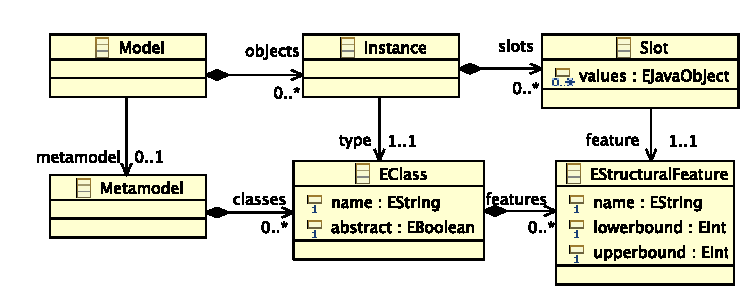
\includegraphics[scale=0.75]{5.Implementation/cope_mm.pdf}
  \caption{Simplification of the metamodel-independent representation used by COPE, based on \cite{herrmannsdoerfer09cope}.}
  \label{fig:cope_mmi}
\end{figure}

Listing~\ref{lst:cope} shows the COPE model migration strategy for the Petri net example given above\footnote{In Listing~\ref{lst:cope}, some of the concrete syntax has been changed in the interest of readability.}. Most notably, slots for features that no longer exist must be explicitly \texttt{unset}. In Listing~\ref{lst:cope}, slots are \texttt{unset} on four occasions, once for each feature that exists in the original metamodel but not the evolved metamodel. Namely, these features are: \texttt{src} and \texttt{dst} of \texttt{Transition} and of \texttt{Place}. Failing to \texttt{unset} slots that do not conform with the evolved metamodel causes migration to fail with an error.

\begin{lstlisting}[caption=Petri nets model migration in COPE, label=lst:cope, language=COPE]
for (transition in Transition.allInstances) {
  for (source in transition.unset('src')) {
    def arc = petrinets.PTArc.newInstance()
    arc.src = source;  arc.dst = transition;
    arc.net = transition.net
  }

  for (destination in transition.unset('dst')) {
    def arc = petrinets.TPArc.newInstance() 
    arc.src = transition; arc.dst = destination;
    arc.net = transition.net
  }
}

for (place in Place.allInstances) {
  place.unset('src');  place.unset('dst');
}
\end{lstlisting}


\subsection{Analysis}
\label{subsec:analysis}
By analysing existing approaches to managing developer-driven co-evolution, requirements were derived for Epsilon Flock, a domain-specific language for specifying and executing model migration. The derivation of the requirements for Epsilon Flock is now summarised, by considering two dimensions: the source-target relationship of the language used for specifying migration strategies and the way in which models are represented during migration. %and the structures provided by the language for specifying and re-using migration strategies.


\subsubsection{Source-Target Relationship}
New target transformation languages (Section \ref{subsubsec:m2m}) require code for explicitly copying from the original to the evolved metamodel those model elements that are unaffected by the metamodel evolution. In contrast, model migration strategies written in COPE (Section~\ref{subsubsec:cope}) must explicitly unset any data that is not to be copied from the original to the migrated model. The Ecore2Ecore approach (Section~\ref{subsubsec:ecore2ecore}) does not require explicit copying or unsetting code. Instead, the relationship between original and evolved metamodel elements is captured in a mapping model specified by the metamodel developer. The mapping model can be configured by hand or, in some cases, automatically derived. 

In each case, extra effort is required when defining a migration strategy due to the way in which the co-evolution approach relates source (original) and target (migrated) model elements. This observation led to the following requirement: \emph{Epsilon Flock must \textbf{automatically} copy every model element that conforms to the evolved metamodel from original to migrated model, and must not automatically copy any model element that does not conform to the evolved metamodel from original to migrated model.}


\subsubsection{Model Representation}
When using the Ecore2Ecore approach, model elements that do not conform to the evolved metamodel are accessed via XMI. Consequently, the metamodel developer must be familiar with XMI and must perform tasks such as dereferencing URI fragments (Listing~\ref{lst:java}) and type conversion. With COPE and the Epsilon Transformation Language, models are loaded using a modelling framework (and so migration strategies need not be concerned with the representation used to store models). Consequently, the following requirement was identified: \emph{Epsilon Flock must not expose the underlying representation of original or migrated models.}

To apply co-evolution operators, COPE requires the metamodel developer to use a specialised metamodel editor, which can manipulate only metamodels defined with EMF. Like, the Ecore2Ecore approach, COPE can be used only to manage co-evolution for models and metamodels specified with EMF. Tight coupling to EMF allows the Ecore2Ecore approach to schedule migration automatically, during model loading. To better support integration with modelling frameworks other than EMF, the following requirement was derived: \emph{Epsilon Flock must be loosely coupled with modelling frameworks and must not assume that models and metamodels will be represented in EMF.}


% \subsubsection{Re-use of migration strategies}
% To produce a suitable migration strategy, each approach requires some effort on the part of the metamodel developer during metamodel evolution. As we discuss more thoroughly in \cite{rose09analysis}, there is a trade-off between the amount of effort required and the flexibility of the approach. 
% 
% COPE seeks to reduce the effort required to express a migration strategy with co-evolutionary operators, which specify re-usable fragments of a migration strategy. With COPE, co-evolutionary operators are applied to perform metamodel evolution and later used to automatically generate a corresponding migration strategy. To apply co-evolution operators, COPE requires the metamodel developer to use a specialised metamodel editor and therefore it is not clear whether operator-based co-evolution can be used with all categories of metamodel editing tool, as we discuss more thoroughly in \cite{rose09analysis}.
% 
% The Ecore2Ecore approach and Epsilon Transformation Language do not require metamodel evolution to occur in a specialised editor and do not provide structures for specifying or re-using migration strategy fragments.
% 
% No existing approach investigates whether it is possible to provide re-usable migration strategy fragments without requiring a specialised metamodel editor. To explore this, the following requirements were derived:  \emph{Epsilon Flock must provide re-usable structures for expressing commonly occurring fragments of migration strategies. Application of the re-usable structures must not require a specialised metamodel editor.}


\subsection{Implementation}
\label{subsec:flock_implementation}
Driven by the analysis presented above, Epsilon Flock (subsequently referred to as Flock) was designed and implemented. Flock is a domain-specific language for specifying and executing model migration strategies. Flock uses a model connectivity framework, which decouples migration from the representation of models and provides compatibility with several modelling frameworks. Flock automatically maps each element of the original model to an equivalent element of the migrated model using a novel conservative copying algorithm and user-defined migration rules (Section~\ref{subsubsec:conservative_copying}).


\subsection{The Epsilon Platform}
Before presenting Flock, it is necessary to revisit some details of the Epsilon \cite{kolovos09thesis} platform, which was introduced in Section~\ref{subsec:epsilon}. Epsilon, a component of the Eclipse GMT project \cite{gmt}, provides infrastructure for implementing uniform and interoperable model management languages, for performing tasks such as model merging, model transformation and inter-model consistency checking. 

The core of the platform is the Epsilon Object Language (EOL) \cite{kolovos06eol}, a reworking and extension of OCL that includes the ability to update models, conditional and loop statements, statement sequencing, and access to standard I/O streams. EOL provides mechanisms for reusing sections of code, such as user-defined operators along with modules and import statements. The Epsilon task-specific languages are built atop EOL, giving highly efficient inheritance and reuse of features.

\subsection{Flock}
Flock is a rule-based transformation language that mixes declarative and imperative parts. Its style is inspired by hybrid model-to-model transformation languages such as the Atlas Transformation Language \cite{jouault05transforming} and the Epsilon Transformation Language \cite{kolovos08etl}. Flock has a compact syntax. Much of its design and implementation is focused on the runtime. The way in which Flock relates source to target elements is novel; it is neither a new nor an existing target relationship. 

\subsubsection{Abstract Syntax}
\label{subsubsec:abstract_syntax}
As illustrated by Figure~\ref{fig:abstract_syntax}, Flock migration strategies are organised into modules (\texttt{Fl\-ockMo\-du\-le}), which inherit from EOL modules (\texttt{Eo\-lMod\-ule}), which provides support for module reuse with import statements and user-defined operations. Modules comprise any number of rules (\texttt{Ru\-le}). Each rule has an original metamodel type (\texttt{or\-ig\-in\-alTy\-pe}) and can optionally specify a \texttt{gu\-ard}, which is either an EOL statement or a block of EOL statements. \texttt{Mi\-gr\-ateRu\-le}s must specify an evolved metamodel type (\texttt{ev\-ol\-vedTy\-pe}) and/or a \texttt{bo\-dy} comprising a block of EOL statements.

\begin{figure}
  \centering
  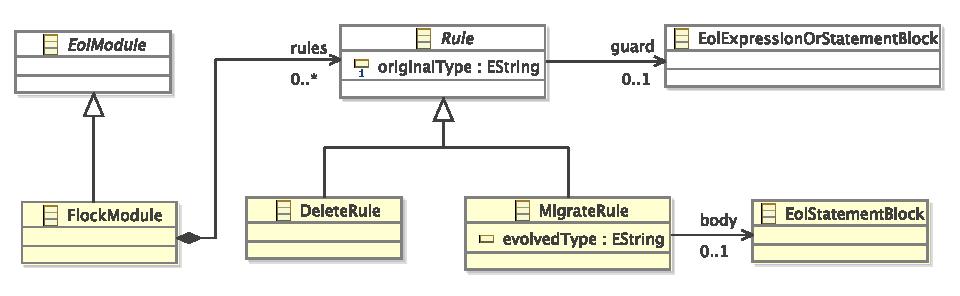
\includegraphics[scale=0.75]{5.Implementation/flock_abstract_syntax.pdf}
  \caption{The abstract syntax of Flock.}
  \label{fig:abstract_syntax}
\end{figure}

\subsubsection{Concrete Syntax}
\label{subsubsec:concrete_syntax}

Listing~\ref{lst:flock_concrete_syntax} shows the concrete syntax of migrate and delete rules. All rules begin with a keyword indicating their type (either \texttt{migrate} or \texttt{delete}), followed by the original metamodel type. Guards are specified using the \texttt{when} keywords. Migrate rules may also specify an evolved metamodel type using the \texttt{to} keyword and a \texttt{body} as a (possibly empty) sequence of EOL statements.

Note there is presently no create rule. In Flock, the creation of new model elements is usually encoded in the imperative part of a migrate rule specified on the containing type.

\begin{lstlisting}[float=tbp, caption=Concrete syntax of migrate and delete rules., label=lst:flock_concrete_syntax, language=Flock]
migrate <originalType> (to <evolvedType>)?
(when (:<eolExpression>)|({<eolStatement>+}))? {
	<eolStatement>*
} 

delete <originalType>
(when (:<eolExpression>)|({<eolStatement>+}))?
\end{lstlisting}

\subsubsection{Execution Semantics}
A Flock module has the following behaviour when executed:

\begin{enumerate}
	\item For each original model element, \texttt{e}:
	\subitem Identify an applicable rule, \texttt{r}. To be applicable for \texttt{e}, a rule must have as its original type the metaclass (or a supertype of the metaclass) of \texttt{e} and the guard part of the rule must be satisfied by \texttt{e}.
	\subitem When no rule can be applied, a default rule is used, which has the metaclass of \texttt{e} as its original type, and an empty body.
	
	\item For each mapping between original model element, \texttt{e}, and applicable delete rule, \texttt{r}:
	\subitem Do nothing.
	
	\item For each mapping between original model element, \texttt{e}, and applicable migrate rule, \texttt{r}:
	\subitem Create an equivalent model element, \texttt{e'} in the migrated model. The metaclass of \texttt{e'} is determined from the \texttt{evolvedType} (or the \texttt{originalType} when no \texttt{evolvedType} has been specified) of \texttt{r}.
	\subitem Copy the data contained in \texttt{e} to \texttt{e'} (using the \emph{conservative copy} algorithm described in the sequel).

	\item For each mapping between original model element, \texttt{e}, applicable migrate rule, \texttt{r}, and equivalent model element, \texttt{e'}:
	\subitem Execute the body of \texttt{r} binding \texttt{e} and \texttt{e'} to variables named \texttt{original} and \texttt{migrated}, respectively.
\end{enumerate}


\subsubsection{Conservative Copying}
\label{subsubsec:conservative_copying}
% TODO A detailed example of conservative copy + equivalence establishment might be useful
Flock contributes an algorithm, termed \emph{conservative copy}, that copies model elements from original to migrated model only when those model elements conform to the evolved metamodel. Because of its conservative copy algorithm, Flock is a hybrid of new target and existing target transformation languages. This section discusses the conservative copying algorithm in more detail.

The algorithm operates on an original model element, \texttt{o}, and its equivalent model element in the migrated model, \texttt{e}. When \texttt{o} has no equivalent in the migrated model (for example, when a metaclass has been removed and the migration strategy specifies no alternative metaclass), \texttt{o} is not copied to the migrated model. Otherwise, conservative copy is invoked for \texttt{o} and \texttt{e}, proceeding as follows:

\begin{itemize}
	\item For each metafeature, \texttt{f} for which \texttt{o} has specified a value
		\subitem Locate a metafeature in the evolved metamodel with the same name as \texttt{f} for which \texttt{e} may specify a value.
			\subsubitem When no equivalent metafeature can be found, do nothing.
			\subsubitem Otherwise, copy to the migrated model the original value (\texttt{o.f}) only when it conforms to the equivalent metafeature
\end{itemize}

The definition of conformance varies over modelling frameworks. Typically, conformance between a value, \texttt{v}, and a feature, \texttt{f}, specifies at least the following constraints:

\begin{itemize}
	\item The size of \texttt{v} must be greater than or equal to the lowerbound of \texttt{f}.
	\item The size of \texttt{v} must be less than or equal to the upperbound of \texttt{f}.
	\item The type of \texttt{v} must be the same as or a subtype of the type of \texttt{f}.
\end{itemize}


Epsilon includes a model connectivity layer (EMC), which provides a common interface for accessing and persisting models. Currently, EMC provides drivers for several modelling frameworks, permitting management of models defined with EMF, the Metadata Repository (MDR), Z or XML. To support migration between metamodels defined in heterogenous modelling frameworks, EMC was extended during the development of Flock. The connectivity layer now provides a conformance checking service. Each EMC driver was extended to include conformance checking semantics specific to its modelling framework. Flock implements conservative copy by delegate conformance checking responsibilities to EMC. 

Finally, some categories of model value must be converted before being copied from the original to the migrated model. Again, the need for and semantics of this conversion varies over modelling frameworks. Reference values typically require conversion before copying. In this case, the mappings between original and migrated model elements maintained by the Flock runtime can be used to perform the conversion. In other cases, the target modelling framework must be used to perform the conversion, such as when EMF enumeration literals are to be copied.


\subsubsection{Development and User Tools}
As discussed in Section~\ref{sec:analysing_existing_techniques}, models and metamodels are typically kept separate. Flock migration strategies can be distributed by the metamodel developer in two ways. An extension point defined by Flock provides a generic user interface for migration strategy execution. Alternatively, metamodel developers can elect to build their own interface, delegating execution responsibility to \texttt{FlockModule}. We anticipate the latter to be useful for production environments using model or source code management repositories.


\subsection{Example}
The exemplar Petri net metamodel evolution is now revisited to demonstrate the basic functionality of Flock. In Listing~\ref{lst:flock}, \texttt{Net}s and \texttt{Place}s are migrated automatically. Unlike the ATL migration strategy (Listing~\ref{lst:atl}), no explicit copying rules are required. Compared to the COPE migration strategy (Listing~\ref{lst:cope}), the Flock migration strategy does not explicitly unset the original \texttt{src} and \texttt{dst} features of \texttt{Transition}.

\begin{lstlisting}[caption=Petri nets model migration in Flock, label=lst:flock, language=Flock]
migrate Transition {
  for (source in original.src) {
    var arc := new Migrated!PTArc;
    arc.src := source.equivalent();  arc.dst := migrated;
    arc.net := original.net.equivalent();
  }

  for (destination in original.dst) {
    var arc := new Migrated!TPArc;
    arc.src := migrated;  arc.dst := destination.equivalent();
    arc.net := original.net.equivalent();
  }
}
\end{lstlisting}

Table~\ref{tab:differences} illustrates several characterising differences between Flock and the related approaches presented in Section~\ref{subsec:co-evo_example}. Due to its conservative copying algorithm, Flock is the only approach to provide both automatic copying and unsetting. Automatic copying is significant for metamodel evolutions with a large number of unchanging features.

All of the approaches considered in Table~\ref{tab:differences} support EMF, arguably the most widely used modelling framework. The Ecore2Ecore approach, however, requires migration to be encoded at the level of the underlying model representation XMI. Both Flock and ATL support other modelling technologies, such as MDR and XML. However, ATL does not automatically copy model elements that have not been affected by metamodel changes. Therefore, migration between models of different technologies with ATL requires extra statements in the migration strategy to ensure that the conformance constraints of the target technology are satisfied. Because it delegates conformance checking to an EMC driver, Flock requires no such checks.

\begin{table}[b]
	\caption{Properties of model migration approaches}
	\centering
	\begin{tabular}{|c|c|c|c|}
		\hline
		             & \textbf{Automatic copy} & \textbf{Automatic unset} & \textbf{Modelling technologies} \\
		\hline
		\textbf{Ecore2Ecore}  & \tick             & \cross              & XMI                    \\
		\hline
		\textbf{ATL}          & \cross            & \tick               & EMF, MDR, KM3, XML     \\
		\hline
		\textbf{COPE}         & \tick             & \cross              & EMF                    \\
		\hline
		\textbf{Flock}        & \tick             & \tick               & EMF, MDR, XML, Z       \\
		\hline
	\end{tabular}
	\label{tab:differences}
\end{table}

A more thorough examination of the similarities and differences between Flock and other migration strategy languages is provided in Chapter~\ref{Evaluation}.


\section{Chapter Summary}
To be completed.
